\documentclass[aspectratio=169]{beamer}

\mode<presentation>
{
  \usetheme{default}
  \usecolortheme{seahorse}
  \usefonttheme{professionalfonts}
  \setbeamertemplate{navigation symbols}{}
  \setbeamertemplate{caption}[numbered]
  \setbeamertemplate{footline}[frame number]
}

\usepackage[utf8x]{inputenc}
\usepackage{graphicx}
\usepackage{physics}
\usepackage{caption}
\usepackage{subcaption}
\usepackage{xcolor}
\usepackage{physics}
\usepackage{amsmath}
\usepackage{tikz}
\usepackage{mathdots}
\usepackage{yhmath}
\usepackage{cancel}
\usepackage{color}
\usepackage{siunitx}
\usepackage{array}
\usepackage{multirow}
\usepackage{amssymb}
\usepackage{gensymb}
\usepackage{tabularx}
\usepackage{extarrows}
\usepackage{booktabs}
\usetikzlibrary{fadings}
\usetikzlibrary{patterns}
\usetikzlibrary{shadows.blur}
\usetikzlibrary{shapes}



\title[quali_slides]{\\ Optimization of SIRIUS nonlinear dynamics}

\author{Matheus Melo Santos Velloso \\{\small student}\\
\vspace{0.5cm}
Dr. Liu Lin\\
Prof. Dr. Antonio Rubens Castro de Britto \\ {\small advisors}}

\institute{Gleb Wataghin Institute of Physics - University of Campinas\\ Accelerator Physics Group (FAC) -  Brazilian Syncrhotron Laboratory (LNLS)}

\date{May 2023}

\AtBeginSection[]
{
    \begin{frame}
         \tableofcontents[currentsection]
   \end{frame}
}

\begin{document}
\maketitle
\begin{frame}{Contents}
    \tableofcontents
\end{frame}

\section{Introduction}
\begin{frame}{SIRIUS}
    \begin{minipage}{0.45\textwidth}
        \begin{figure}
            \centering
            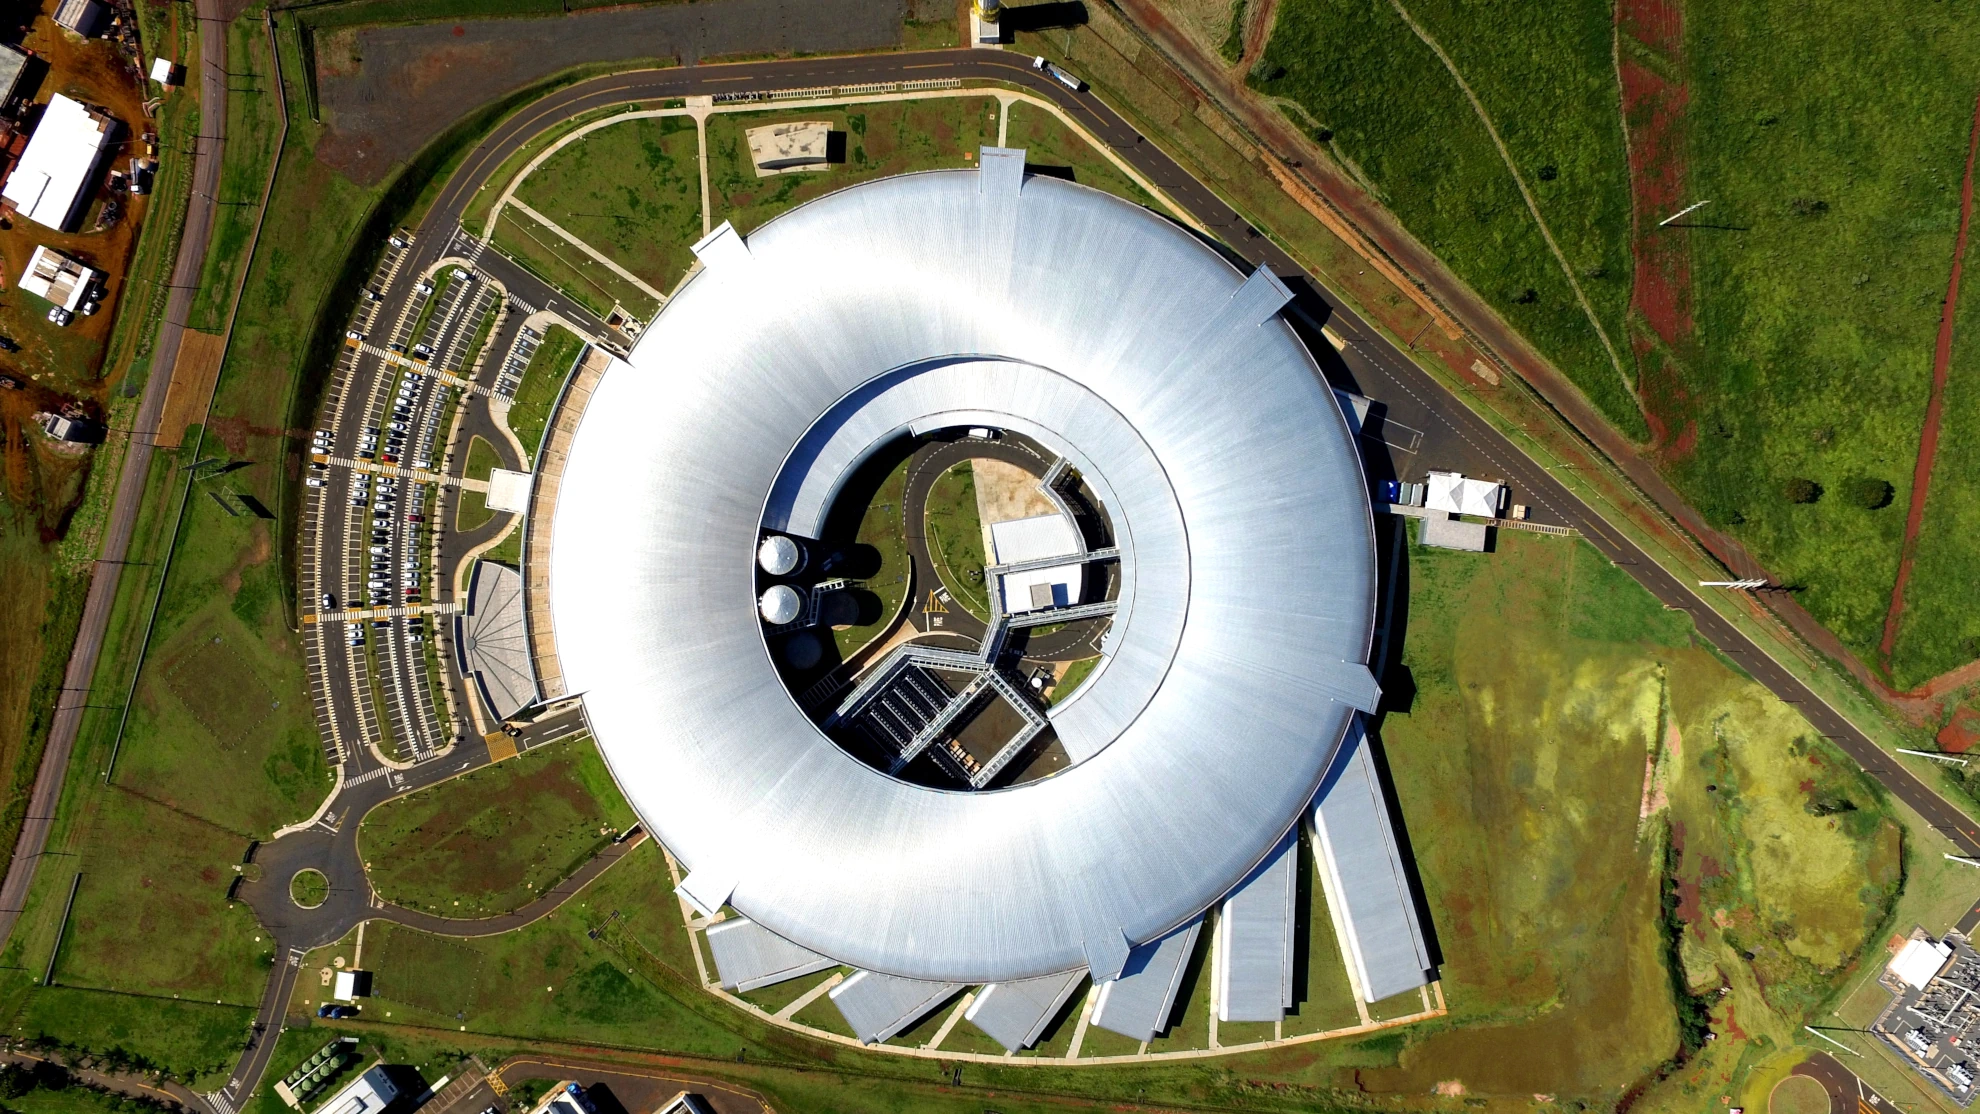
\includegraphics[width=\textwidth]{f1.png}
        \end{figure}
    \end{minipage}
    \hfill
    \begin{minipage}{0.45\textwidth}
        \begin{itemize}
            \item 4th generation storage ring-based synchrotron light source
            \item LINAC, booster, storage ring
            \item Storage ring: $518~\unit{\m}$ in circumf, $3~\unit{GeV}$, nominal energy
            \item $100~\unit{mA}$ current, top-up injection mode
        \end{itemize}
    \end{minipage}
\end{frame}
\begin{frame}{Storage rings}
    \begin{figure}
        \centering
        \includegraphics[scale=0.3]{storage_ring.png}
    \end{figure}
% \begin{minipage}
%     \begin{figure}
%         \centering
%         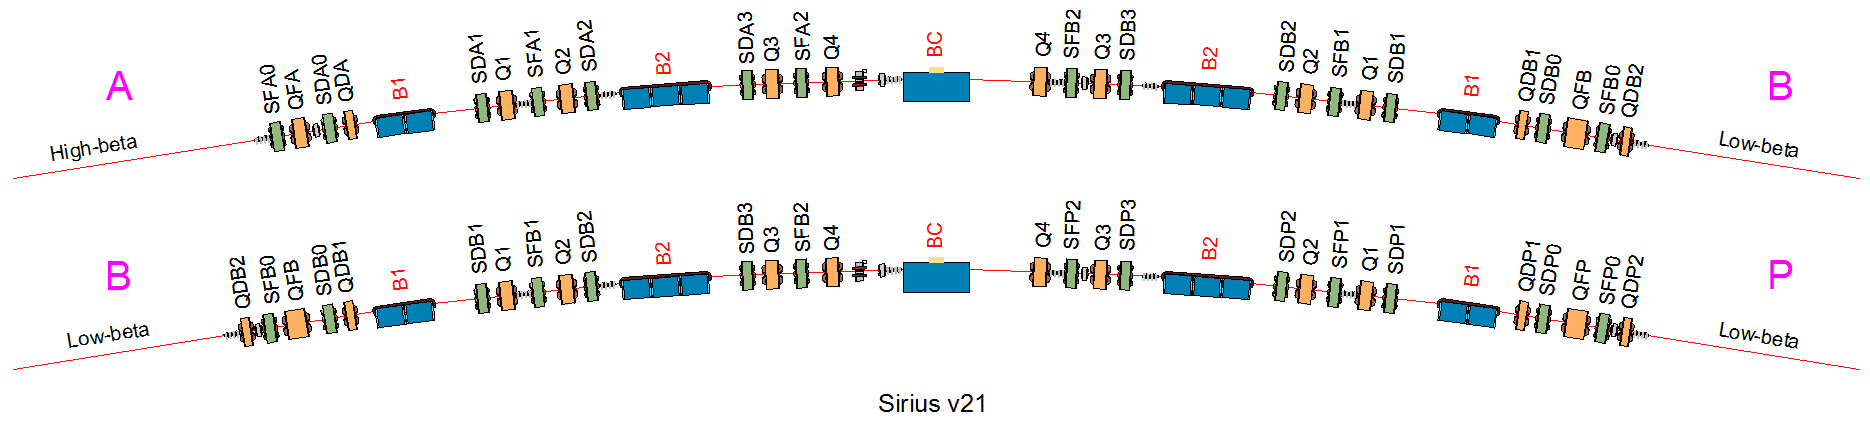
\includegraphics[scale=0.2]{SI_superperiod.png}
%     \end{figure}
% \end{minipage}
\end{frame}

\begin{frame}{The dissertation problem}
    Off-axis injection scheme
    \begin{figure}
        \centering
        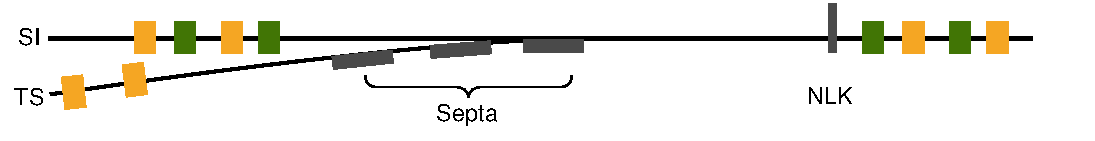
\includegraphics[width=0.7\textwidth]{injection.pdf}
    \end{figure}
    \pause
    \begin{figure}
        \centering
        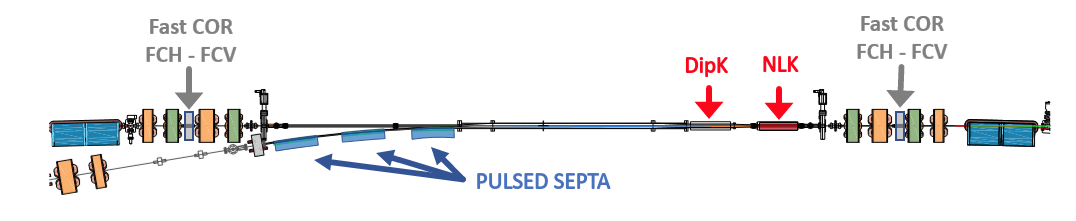
\includegraphics[width=0.7\textwidth]{off_axis_injection.png}
    \end{figure}
\end{frame}
\section{Theoretical background}
\begin{frame}{The Frenet-Serret Frame}
    \begin{minipage}{0.45\textwidth}
        \begin{figure}
            \centering
            \includegraphics[width=\textwidth]{frenetserret.png}
            \caption*{Lab and Frenet-Serret Frames\\ {\tiny  from \textit{Beam-based correction and optimization}, X. Huang}}
        \end{figure}
    \end{minipage}
    \hfill
    \begin{minipage}{0.45\textwidth}
        Defined by
        $$\vu{s}=\dv{\vb{r}_{0}}{s}, \quad \vu{x}=-\rho\dv{\vu{s}}{s}$$
        $$\vu{y} =  \vu{x}\times\vu{s}$$

        satisfying
    $$\dv{\vu{s}}{s}=-\frac{1}{\rho(s)}\vu{x}, \quad\dv{\vu{x}}{s}=\frac{1}{\rho(s)}\vu{s}$$
    $$\dv{\vu{y}}{s}=0$$
    \end{minipage}

        {\tiny J. V. José, E. J. Saletan.\textit{ Classical Dynamics - A contemporary Approach}; S. Y. Lee. \textit{Accelerator Physics}. }
\end{frame}
\begin{frame}{Magnetic fields}
    \begin{minipage}{0.59\textwidth}
        \begin{itemize}
            \item Horizontal Dipole:\\
                   $$ B_x = 0, \quad B_y = B_0$$
            \item Normal quadrupole\\
                  $$B_x = B_1 y, \quad B_y = B_1 x$$
            \item Normal sextupole\\
                  $$B_x = B_2xy, \quad B_y = \frac{1}{2}B_2(x^2 - y^2)$$
        \end{itemize}
    \end{minipage}
    \hfill
    \begin{minipage}{0.39\textwidth}
    \begin{figure}
        \centering
        \includegraphics[height=0.7\textheight]{fields.png}
    \end{figure}
    \end{minipage}
    \pause
    Magnetic rigidity normalization:
        $$G(s) = \frac{B_0(s)}{B\rho}, \quad K(s) = \frac{B_1(s)}{B\rho}, \quad S(s) = \frac{B_2(s)}{B\rho}$$
\end{frame}
\begin{frame}{Equations of motion}
The set of canonical variables for the transverse dynamics in a paraxial approximation will be $(x,p_{x},y , p_{y})$. Where
$$\begin{cases} p_{x}=\frac{P_x}{P_0}\approx x^\prime(1+\delta)\\p_{y}=\frac{P_y}{P_0}\approx y^\prime (1+\delta)\end{cases},  \quad \delta = \frac{P-P_{0}}{P_{0}}$$
\pause
Equations of motion
$$
x^{\prime \prime}=-\frac{(1+G x)^{2}}{1+\delta} \frac{B_{y}}{B \rho}+G(1+G x),
\quad
y^{\prime \prime}=\frac{(1+G x)^{2}}{1+\delta} \frac{B_{x}}{B \rho}, \quad G(s) = \frac{1}{\rho(s)}
$$
\end{frame}
\begin{frame}{Linear dynamics}
\begin{minipage}{0.49\textwidth}
    Equations of motion in the linear approx.
    \begin{equation*}
        x^{\prime\prime}+(G^2+K)x=G\delta,
    \end{equation*}
    \begin{equation*}
        y^{\prime\prime}-Ky=0,
    \end{equation*}
    \pause
    On-momentum particles: Hill's equations
    \begin{equation*}
        u^{\prime\prime}+K_u(s)u = 0,
    \end{equation*}
    \pause
    with $u=x,y$ and
    $$K_x = G^2 + K,$$ $$K_y = - K.$$
\end{minipage}
\hfill
\pause
\begin{minipage}{0.49\textwidth}
    \begin{figure}
        \centering
        \includegraphics[width=\textwidth]{g_k_SIRIUS.pdf}
    \end{figure}
\end{minipage}
\end{frame}
\begin{frame}{Pseudoharmonic solution}
Amplitude-phase solution to Hill's equation:
    \begin{equation*}
        u(s) = \sqrt{2\beta_u(s) J_u}\cos(\phi_u(s) + \phi_0),
    \end{equation*}
    \pause
    where $\beta_u(s)$ must satify
    \begin{equation*}
        \frac{1}{2}\beta_{u}^{\prime\prime}+\beta_{u} K_u(s) - \frac{1}{\beta_{u}}\qty(\frac{1}{4}\beta_{u}^{\prime 2} + 1 ) = 0, \quad
            \begin{cases}
                \beta_{u}(0) = \beta_{u}(L)\\ \beta_{u}^{\prime}(0) = \beta_{u}^{\prime}(L)
            \end{cases}
    \end{equation*}
    \pause
    \begin{minipage}{0.49\textwidth}
        the phase advance is
            \begin{equation*}
                \phi_u(s) = \int_{0}^{s}\frac{1}{\beta_u(\sigma)}\dd\sigma
            \end{equation*}
    \end{minipage}
    \hfill
    \begin{minipage}{0.49\textwidth}
        and the \textit{tune} is the \# of cycles per rev.
        \begin{equation*}
            \nu=\frac{1}{2\pi}\int_{s}^{s+L}\frac{\dd \sigma}{\beta(\sigma)}\equiv\frac{1}{2\pi}\oint\frac{\dd s}{\beta(s)}
        \end{equation*}
    \end{minipage}
\end{frame}
\begin{frame}{The beta functions}
        The amplitude function for a SIRIUS superperiod
    \begin{figure}
        \centering
        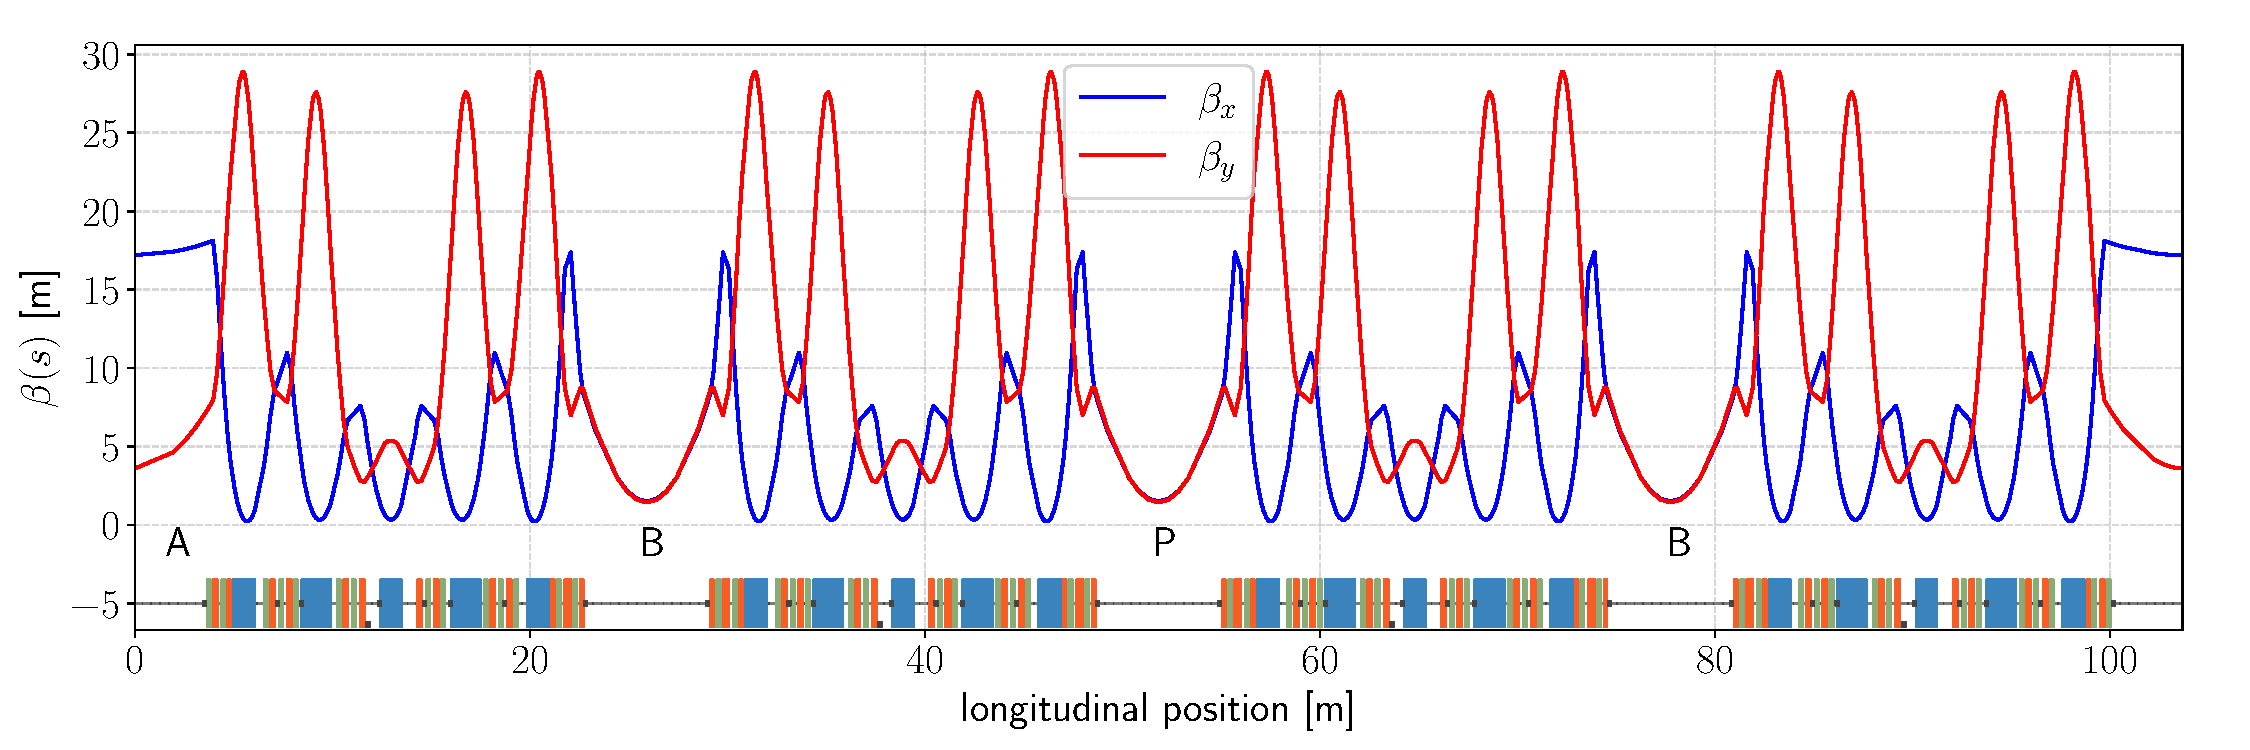
\includegraphics[width=\textwidth]{beta_functions.pdf}
    \end{figure}
\end{frame}
\begin{frame}{Phase flows in the linear approximation}
    \begin{minipage}{0.45\textwidth}
        % \begin{equation*}
        %     u(s) = \sqrt{2\beta_u(s) J_u}\cos(\phi_u(s) + \phi_0)
        % \end{equation*}
        % \begin{equation*}
        %     \begin{aligned}{}
        %         u^{\prime}(s) & =-\sqrt{\frac{2J_u}{\beta_u(s)}}\Big{[}\alpha_u(s)\cos(\phi_u(s)-\phi_0)\\ &\quad \quad \quad  \quad -\sin(\phi_u(s)-\phi_0)\Big{]}
        %     \end{aligned}
        % \end{equation*}
        Defining $\alpha_u = \frac{\beta_u^\prime}{2}$  \& $\gamma_u = \frac{(1+\alpha_u^2)}{\beta_u}$:

        $$2J_u=\gamma u^{2}+2\alpha u u^{\prime}+\beta u^{\prime2}$$
    \end{minipage}
    \hfill
    \pause
    \begin{minipage}{0.45\textwidth}
        \begin{figure}
        \centering
        \includegraphics[width=\textwidth]{ellipse.png}
        \end{figure}{}
    \end{minipage}
\end{frame}
\begin{frame}{Dispersion fuction}
    Off-momentum particle EOM
    \begin{equation*}
        x^{\prime\prime}+(G^2+K)x=G\delta
    \end{equation*}
    \pause
    Solution $x=x_\beta+ x_\delta = x_\beta+ \eta(s)\delta $, \pause where $\eta(s)$ satisfies
    \begin{equation*}
        \eta^{\prime\prime}+(G^2+K)\eta=G\quad
        \begin{cases}
            \eta(0) = \eta(L)\\
            \eta^\prime(0) = \eta^\prime(L)
        \end{cases}
    \end{equation*}
    \pause
    \begin{figure}
        \centering
        \includegraphics[width=0.8\textwidth]{dispersion.pdf}
    \end{figure}
\end{frame}
\begin{frame}{Linear Optics}
    \begin{figure}
        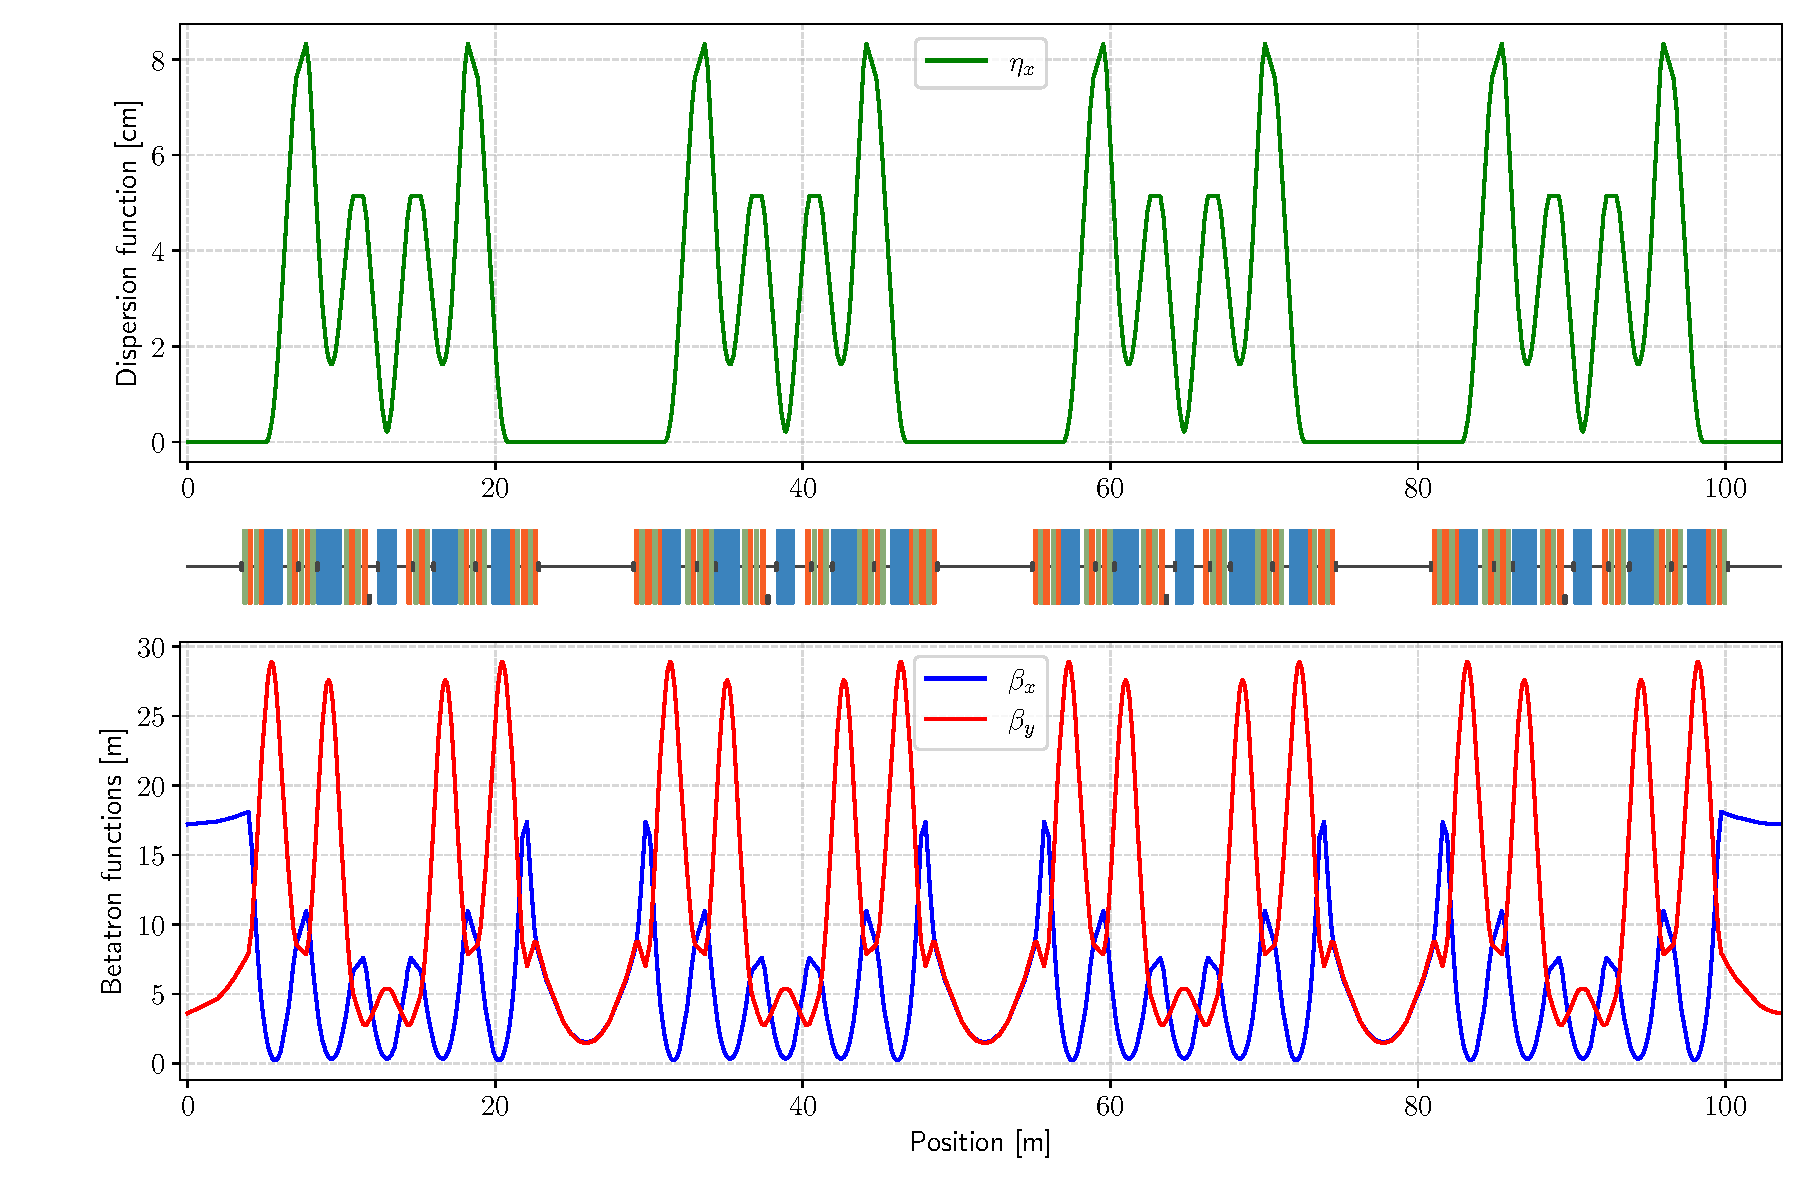
\includegraphics[width=0.8\textwidth]{linear_optics.pdf}
    \end{figure}
\end{frame}

\begin{frame}{Nonlinear Dynamics}
    Forced Hill's equations
    \begin{equation*}
        u^{\prime\prime}+K_u(s)u(s) = f(s)
    \end{equation*}
    % can be cast into a forced Harmonic Oscillator equation
    % \begin{equation*}
    %     \dv[2]{w}{\Phi}+\nu_{u0}^2w = \nu_{u0}^2 \beta_u^{3/2}f(s)
    % \end{equation*}
    % upon the transformations
    % \begin{equation*}
    %     \begin{aligned}
    %         \Phi_u(s)=\frac{1}{\nu_{u0}}\int_0^s \dd\sigma \frac{1}{\beta_u(\sigma)}, \quad
    %         w(s)= \frac{u(s)}{\sqrt{\beta_u(s)}}
    %     \end{aligned}
    % \end{equation*}
%    The use of the Green's function gives
%    \begin{equation}
%        u(s) = \frac{\sqrt{\beta_u(s)}}{2\sin\pi\nu_u}\int_{s}^{s+L} f(\sigma)\sqrt{\beta_u(\sigma)}\cos(\pi\nu_u + \phi_u(s) - \phi_u(\sigma))\dd \sigma.
%    \end{equation}
    where $f(s)$ is expanded in powers of $x$ and $y$ to represent higher multipoles perturbation and coupling effects.
    \vfill
    General features of a nonlinear dynamics:
    \begin{itemize}
        \item Tune-shifts: energy-dependent and amplitude-dependent $$\nu_0 = \nu_{u0} + \xi_u(\delta) \delta + \alpha_{uu} J_u + \alpha_{uv} J_v$$
        \item Resonances
    \end{itemize}
\end{frame}
\begin{frame}{Tune-shifts}
    \begin{figure}
        \centering
        \includegraphics[height=0.8\textheight]{nonlinear_dynamics_phase_tunes.pdf}
    \end{figure}
\end{frame}
\begin{frame}{Ressonances}
    \begin{minipage}{0.48\textwidth}
           If the tunes satisfy
           $$m_x\nu_x+m_y\nu_y=\ell$$
           then we have a $\abs{m_x}+\abs{m_y}$ order resonance.
    \end{minipage}{}
    \hfill
    \begin{minipage}{0.48\textwidth}
        \begin{itemize}
               \item 1st order: integer resonance
               \item 2nd order: $1/2$ integer resonance
               \item 3rd order: $1/3$ integer resonance
           \end{itemize}{}
    \end{minipage}{}

    \begin{figure}
        \centering
        \includegraphics[scale=0.3]{tunes.png}
        \caption*{Up to 2nd, 3rd and 4th order resonances in tune space.}
    \end{figure}{}
\end{frame}{}
\begin{frame}{SIRIUS Dynamic Aperture}
    \begin{minipage}{0.49\textwidth}
        \begin{figure}
            \centering
            \includegraphics[width=\textwidth]{da_xy_model.pdf}
        \end{figure}
    \end{minipage}
    \begin{minipage}{0.49\textwidth}
        \begin{figure}
            \centering
            \includegraphics[width=\textwidth]{da_xy_meas.png}
        \end{figure}
    \end{minipage}
\end{frame}
\begin{frame}{The need for a large Dynamic Aperture}
    Off-axis injection scheme
    \begin{figure}
        \centering
        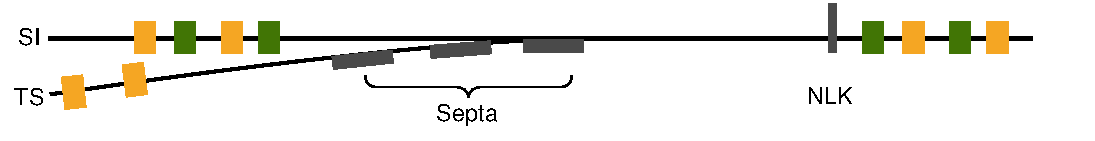
\includegraphics[width=0.7\textwidth]{injection.pdf}
    \end{figure}
    \begin{figure}
        \centering
        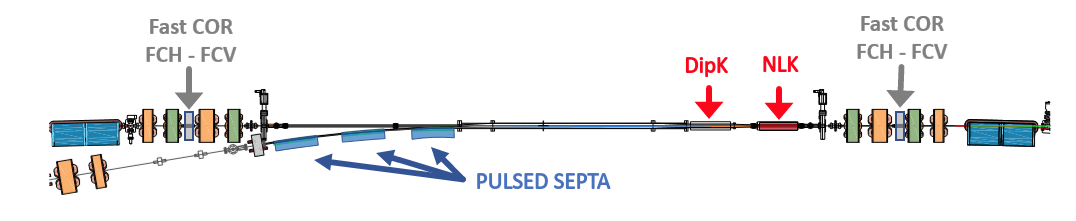
\includegraphics[width=0.7\textwidth]{off_axis_injection.png}
    \end{figure}
\end{frame}
\begin{frame}{The need for a large Dynamic Aperture}
        \begin{figure}
            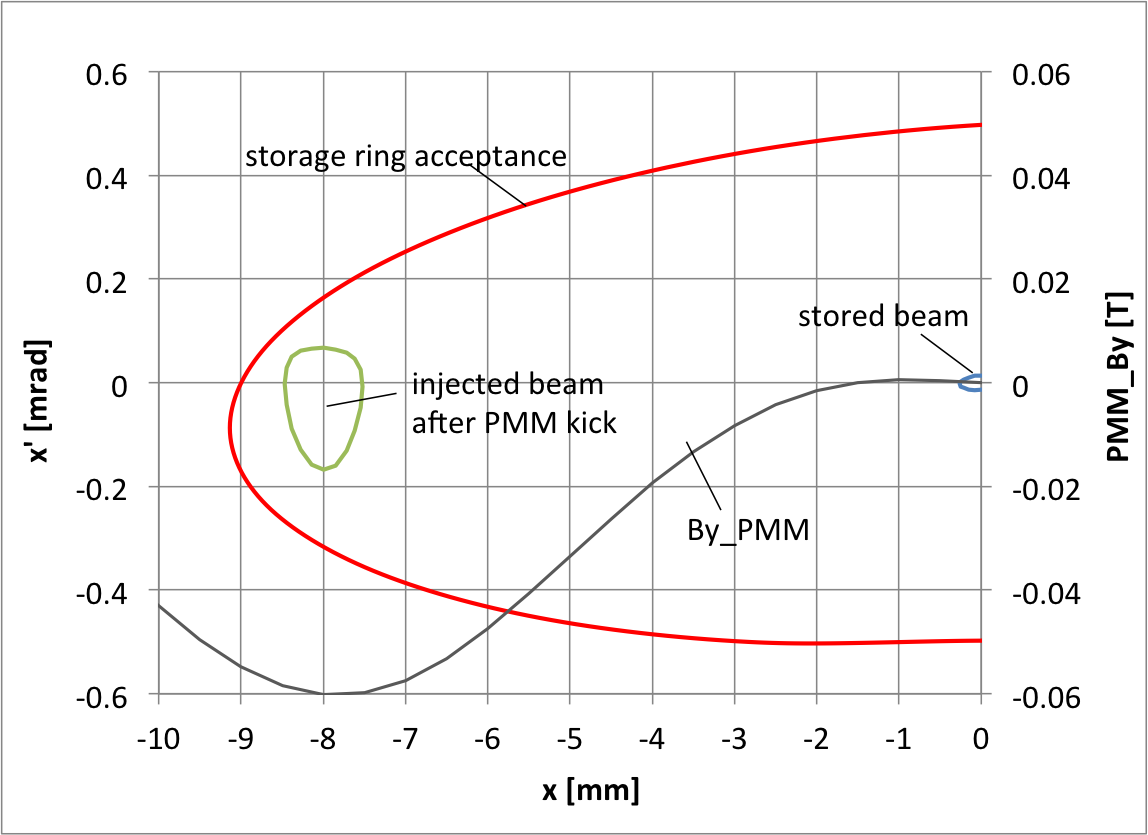
\includegraphics[width=0.7\textwidth]{nlk_phase_space.png}
        \end{figure}
\end{frame}
\section{Online optimization of Dynamic Aperture}
\begin{frame}{Online Optimization Set-up}
    \begin{itemize}
        \item Define the objective function and optimization knobs
    \end{itemize}{}
    \begin{itemize}
        \item Choose optimization algorithm and strategy
    \begin{itemize}
        \item Gradient-based
        \begin{itemize}
            \item Gradient Descent
            \item Gauss-Newton/Levenberg-Marquardt
        \end{itemize}
        \item Gradient-free (direct-, indirect-search)
        \begin{itemize}
            \item Brent's /Parabolic Interpolation Methods/ Golden Section Search
            \item Nelder-Mead downhill simplex
            \item Direction set methods (Powell, RCDS)
            \item Machine Learning / Surrogate models (Gaussian Processes Bayesian Optimzation)
        \end{itemize}
    \end{itemize}{}
    \end{itemize}{}
    \pause
    We need an optimization routine well-suited for \textit{online optimization}: optimization of a measured objective function with no analytical closed form + measurement errors
\end{frame}{}
\begin{frame}{Robust Conjugate Direction Search (RCDS) Algorithm}
    Huang, X. SLAC-PUB-15414. 2013
    \begin{itemize}
    \item Based on Powell's (1964) conjugate directions search
    \item Steps
    \begin{itemize}
        \item Powell's loop
        \item Bracketing
        \item Line search
    \end{itemize}
    \item Extensively used in the accelerator community
    \begin{itemize}
        \item Nonlinear dynamics optimzation
        \begin{itemize}
            \item Dynamic aperture
            \item Momentum acceptance
            \item ADTS
        \end{itemize}
        \item Emittance Minimization
        \item Optics \& steering matching during injection
    \end{itemize}
   \end{itemize}
\end{frame}{}
\begin{frame}{SIRIUS Dynamic Aperture Optimization}
    \begin{minipage}{0.55\textwidth}
        Working point $\nu_x, = 49.08, \nu_y = 14.14$
        \begin{figure}
            \centering
            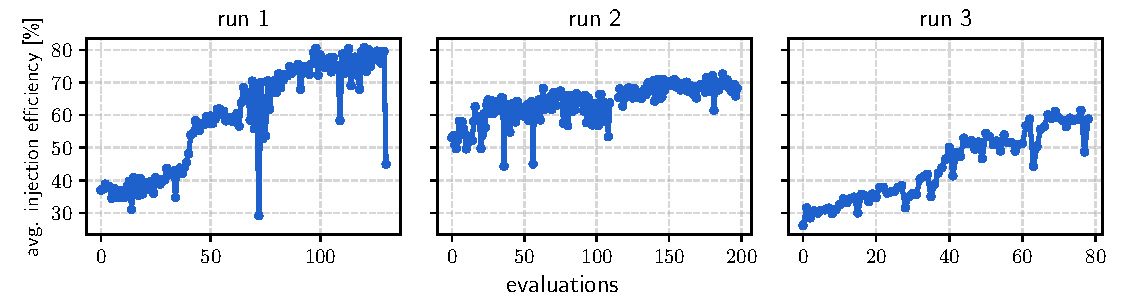
\includegraphics[width=\textwidth]{oldtunes_history.pdf}
            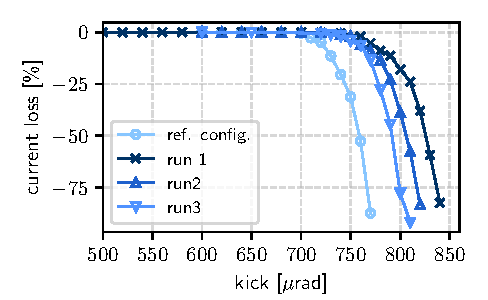
\includegraphics[width = 0.8\textwidth]{WEPL087_f1.pdf}
            \vfill
            \begin{itemize}
                \item injection efficiency: $98\pm1~\%$ run 2
                \item 1 hour reduction in lifetime
            \end{itemize}
        \end{figure}
    \end{minipage}
    \hfill
    \begin{minipage}{0.44\textwidth}
        \begin{figure}
            \centering
            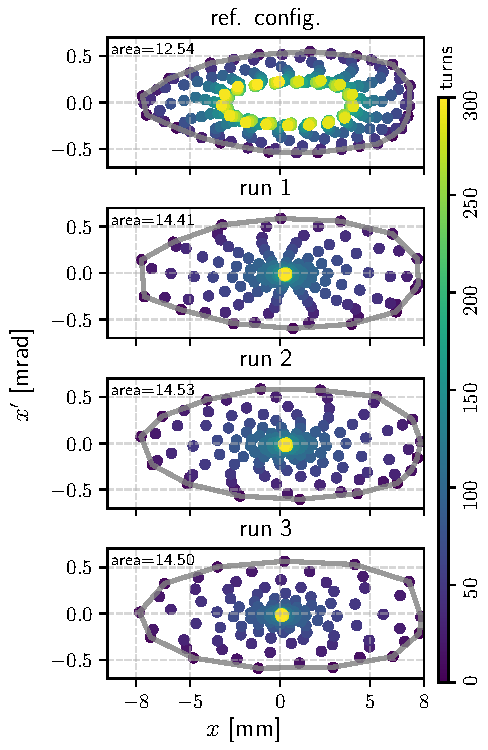
\includegraphics[height=0.9\textheight]{WEPL087_f2.pdf}
        \end{figure}
    \end{minipage}
\end{frame}
% \begin{frame}{SIRIUS Dynamic Aperture Optimization}
%     \begin{minipage}{0.55\textwidth}
%         Working point $\nu_x, = 49.20, \nu_y = 14.25$
%         \begin{figure}
%             \centering
%             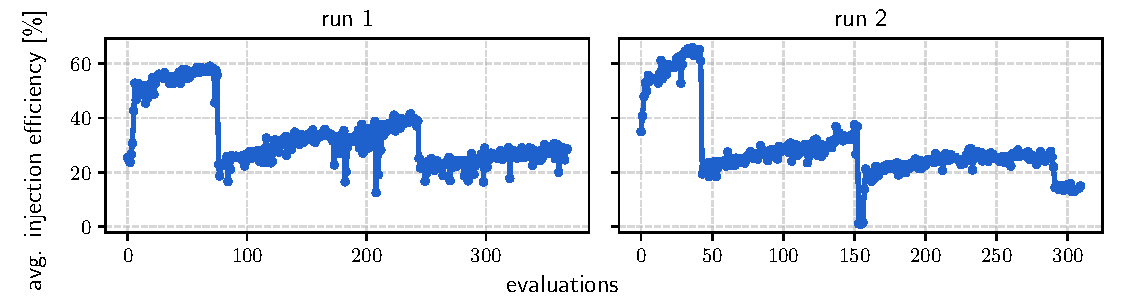
\includegraphics[width=\textwidth]{newtunes_history.pdf}
%             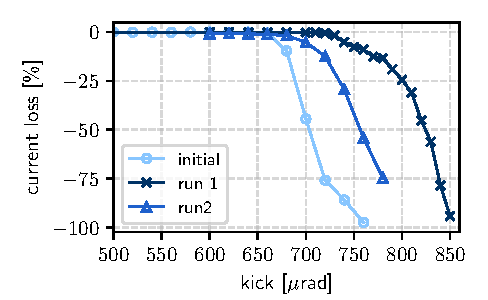
\includegraphics[width = 0.8\textwidth]{WEPL087_f3.pdf}
%             \begin{itemize}
%                 \item injection efficiency: $79\pm3~\%$ run 1
%                 \item no reduction in lifetime
%             \end{itemize}
%         \end{figure}
%     \end{minipage}
%     \hfill
%     \begin{minipage}{0.44\textwidth}
%         \begin{figure}
%             \centering
%             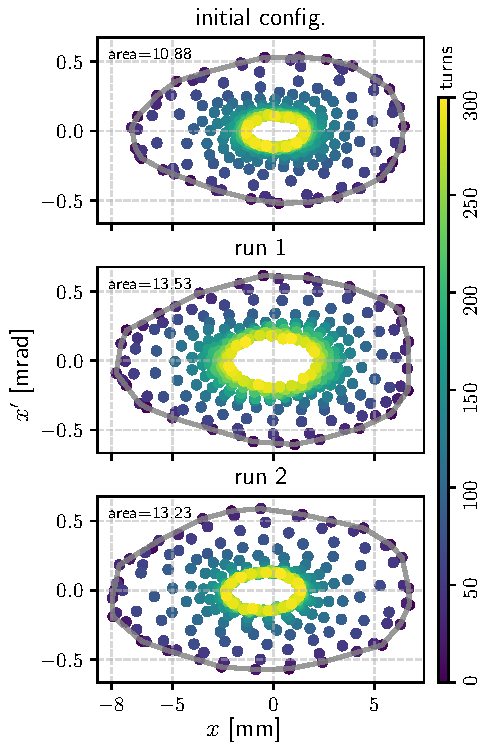
\includegraphics[height=0.9\textheight]{WEPL087_f4.pdf}
%         \end{figure}
%     \end{minipage}
% \end{frame}
% \begin{frame}{SIRIUS Dynamic Aperture Optimization}
%     \begin{minipage}{0.55\textwidth}
%         Working point $\nu_x, = 49.16, \nu_y = 14.22$
%         \begin{figure}
%             \centering
%             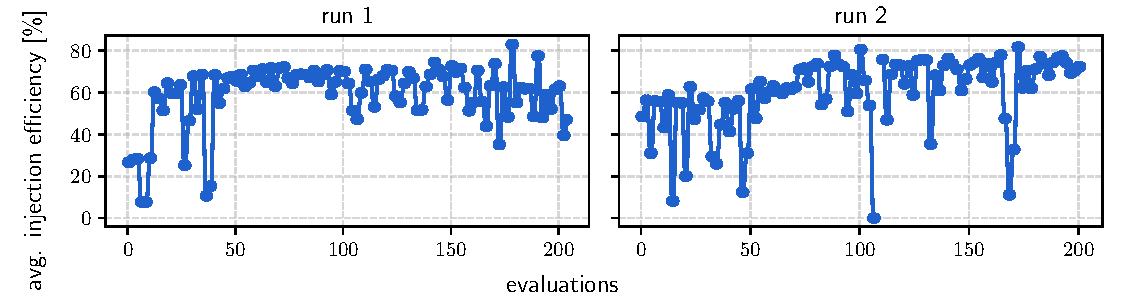
\includegraphics[width=\textwidth]{wp3_history.pdf}
%             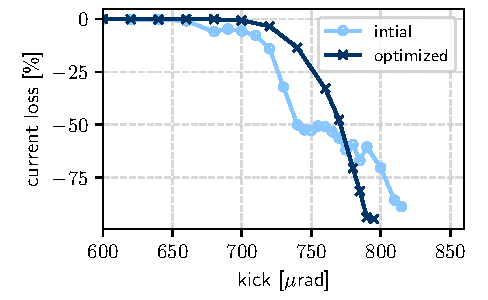
\includegraphics[width = 0.8\textwidth]{wp3_kick_resilience.pdf}
%             \begin{itemize}
%                 \item injection efficiency: $93\pm3~\%$ run 1
%                 \item 1.5 hr reduction in lifetime
%             \end{itemize}
%         \end{figure}
%     \end{minipage}
%     \hfill
%     \begin{minipage}{0.44\textwidth}
%         \begin{figure}
%             \centering
%             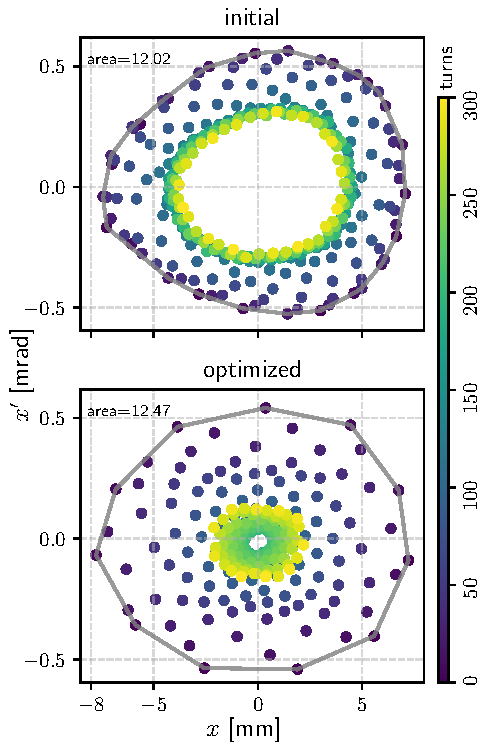
\includegraphics[height=0.9\textheight]{wp3_phase_space.pdf}
%         \end{figure}
%     \end{minipage}
% \end{frame}
\begin{frame}
    Thank you!
\end{frame}
% \begin{frame}{Summary of Activities}
%     Dissertation activities
%     \begin{itemize}
%         \item Beam dynamics studies (03/2022 - 06/2022)
%         \item RCDS code implementation and testing (07-08/2022)
%         \item RCDS tests: Injection Efficiency Optimization with TS PosAng  (09-10/2022)
%         \begin{itemize}
%             \item IV CEC Poster Presentation (11/2022)
%         \end{itemize}
%         \item Initial RCDS tests for DA optimization (12/2022)
%         \item Qualitative studies of optimization in the machine model (01/2023)
%         \item Dr. Xiabiao Huang visit and Online Optimization Experiments (02/2023)
%         \item New working point optimization  (03-05/2023)
%         \item Paper/poster preparation for IPAC'23 (04-05/2023)
%         \begin{itemize}
%             \item M. M. S. Velloso, M. B. Alves, L. Liu, X. R. Resende, F. H. de Sá, X. Huang. \textit{Online Optimization of SIRIUS nonlinear optics}. In \textit{Proc. IPAC'23}. 2023.
%         \end{itemize}
%     \end{itemize}
%     Course credits/academic activities
%     \begin{itemize}
%         \item FI001, FI004 (2022/1);  FI002 (2022/2);  FI195 - 2023/1
%         \item PED C F228 (2023/1)
%     \end{itemize}
% \end{frame}
\section*{Backup}
\begin{frame}{Motion of charged particles in magnetic fields}
    \begin{minipage}{\textwidth}
        \begin{minipage}{0.6\textwidth}
            Circular motion in a uniform field
            \begin{equation*}
                \rho =  \frac{p}{qB}\to B\rho = \frac{p}{q}
            \end{equation*}
        \end{minipage}
        \hfill
        \begin{minipage}{0.39\textwidth}
            \begin{figure}
                \centering
                \includegraphics[width=\textwidth]{uniform_field.png}
            \end{figure}
        \end{minipage}
    \end{minipage}
    \vfill
    \pause
    \begin{minipage}{\textwidth}
        \begin{minipage}{0.6\textwidth}
            Deflection when passing through arbitrary fields
            \begin{equation*}
                \dd{\theta_x} = \frac{\dd{s}}{\rho_x(s)} = \frac{e}{p}B_y(x,y,s)\dd s = \frac{1}{B\rho}B_y(x,y,s)\dd s
            \end{equation*}
            \begin{equation*}
                \dd{\theta_y} = \frac{\dd{s}}{\rho_y(s)} = \frac{e}{p}B_x(x,y,s)\dd s = \frac{1}{B\rho}B_y(x,y,s)\dd s
            \end{equation*}
        \end{minipage}
        \begin{minipage}{0.39\textwidth}
            \begin{figure}
                \centering
                \includegraphics[width=\textwidth]{arbitrary_fields.png}
            \end{figure}
        \end{minipage}
    \end{minipage}
\end{frame}
\begin{frame}{Hamiltonian for relativistic electron}
The dynamics of relativistic electrons influenced by electromagnetic fields $(\Phi, \vb{A})$ is contained in the Hamiltonian
    \begin{equation*}
        H=\sqrt{m^2c^4+(\vb{P}-q\vb{A})^2c^2}+e\Phi,
    \end{equation*}
 $e$ being the elementary charge and $\vb{P}=\vb{p}+e\vb{A}$ the canonical momentum.
\vfill
 \begin{minipage}{0.5\textwidth}
    \begin{itemize}
        \item Frenet-Serret frame coordinates
        \item change of independent variable: $t\to s$
        \item paraxial approximation \& geometric variables
     \end{itemize}
 \end{minipage}
 \hfill
\begin{minipage}{0.49\textwidth}
\begin{figure}
    \centering
    \includegraphics[width=\textwidth]{paraxial.pdf}
\end{figure}
 \end{minipage}
\end{frame}
\begin{frame}{Focusing errors for off-energy particles}
    \begin{figure}
        \centering
        \includegraphics[width=0.5\textwidth]{nat_chrom.png}
    \end{figure}{}
    \pause
    \begin{minipage}{\textwidth}
        EOMs up to $\order{x\delta}$
            \begin{equation*}
                x^{\prime\prime}+(K_x+\Delta K_x)x=0, \quad
                y^{\prime\prime}+(K_y+\Delta K_y)y=0
            \end{equation*}
            \begin{equation*}
                \Delta K_x  \approx - K\delta,\quad
                \Delta K_y =  K\delta
            \end{equation*}
            \pause
            \begin{minipage}{0.49\textwidth}
            $\delta$-induced tune-shift
            \begin{equation*}
                \Delta \nu _u = \mp \frac{1}{4\pi}\oint\beta_u K \delta \dd{s}
            \end{equation*}

        \end{minipage}
        \begin{minipage}{0.49\textwidth}

            chromaticity $\xi = \dv{\nu}{\delta}$
            \begin{equation*}
                \xi_{\text {nat}, u} =\mp \frac{1}{4 \pi} \oint K \beta_u \dd{s}
            \end{equation*}
        \end{minipage}
    \end{minipage}
    \vfill
\end{frame}{}
\begin{frame}{Chromaticity Correction}
    Off-energy particles, to leading order, feel the feed-down quadrupolar error from a sextupole
    $$\Delta K_{u}(s,\delta)=\pm S(s)\eta(s) \delta$$
    The chromaticity then is
    \begin{equation*}
        \xi_{u}=\mp \frac{1}{4\pi}\oint\beta_{u}(K - S\eta)\dd{s}
    \end{equation*}
\end{frame}
\begin{frame}{Chromaticity Jacobian null-space}

\end{frame}
\begin{frame}{SIRIUS Dynamic Aperture}
\begin{figure}
    \centering
    \includegraphics[width=0.5\textwidth]{machine_ensemble_DAs.png}
\end{figure}
\pause
Model predicts $x\sim-10~\unit{mm}$, machine presents $x\sim-8.5~\unit{mm}$
\end{frame}
\begin{frame}{Perturbations}
    General n-th order perturbation
    $$x^{\prime\prime}+K_{x}x = p_{rs}x^{r}y^{s}, \quad r+s\leq n-1$$
    \pause
    Transforming  to $w = x / \sqrt{\beta_x}$ and $v = y / \sqrt{\beta_y}$ leads to
        $$\ddot{w}+\nu_{x,0}^{2}w=\nu^{2}\beta_{x}^{3/2}\beta_{x}^{r/2}\beta_{y}^{s/2}p_{rs}w^{r}v^{s}$$
    \pause
    Assuming $w\approx w_0$, $v\approx v_0$ and Fourier-expanding \pause

    $$\ddot{w}+\nu_{x0}^{2}w=\sum_{\abs{l}\leq r}\sum_{\abs{k}\leq s}\sum_{m} q_{rs}^{(m)}W_{l}V_{k}e^{i(m+l\nu_{0x}+k\nu_{0y})\Phi}$$
    \pause
    Ressonances: $m+l\nu_{0x}+k\nu_{0y} = \nu_{0x} \iff m+(l-1)\nu_{0x}+k\nu_{0y}=0$\\
    \pause

    Similarly, in $y$: $m+\ell\nu_{0x}+\kappa\nu_{y0}=\nu_{y0} \iff m+\ell\nu_{0x}+(\kappa-1)\nu_{y0}=0$.
    $$m_x\nu_{0x}+m_y\nu_{0y}=\ell$$
\end{frame}
\begin{frame}{Integer and half-integer resonances}
    Orbit distortions due to dipolar perturbations $\theta(s)$
\begin{equation*}
    x_{\text{co}}(s) = \frac{\sqrt{\beta(s)}}{2\sin\pi\nu}\int_{s}^{s+L} \theta(\sigma)\sqrt{\beta(\sigma)}\cos(\pi\nu + \phi(s) - \phi(\sigma))\dd \sigma.
\end{equation*}
    Beta-beating due to gradient errors $k(s)$
 \begin{equation*}
    \frac{\Delta \beta(s)}{\beta(s)} = - \frac{1}{2\sin(2\pi\nu_0)}\int_{s}^{s+L}k(\sigma)\cos(2\phi(\sigma)-2\phi(s)-\phi_0)\dd\sigma.
 \end{equation*}
\end{frame}{}
\begin{frame}{Amplitude-dependent tune-shift (ADTS)}
    \begin{equation*}
        \begin{aligned}
            \nu_x & = \nu_{x0} - \frac{1}{4\pi}\int_0^L\beta_x(s)(K-S\eta_x)\delta  \\ & \quad - \frac{1}{64\pi} J_x \int_0^L \dd s \int_s^{s+L}\dd s^\prime \beta_x^{3/2}(s)S(s)\beta_x^{3/2}(s^\prime)S(s^\prime)\qty[
                \frac{3\cos\theta_x}{\sin\pi\nu_{0x}} + \frac{\cos3\theta_x}{\sin3\pi\nu_{0x}}]
        \end{aligned}
    \end{equation*}
    where $\theta_x = \phi_x(s^\prime) - \phi_x(s) - \pi\nu_{0x}$.
\end{frame}
% \begin{frame}{Online Optimization Experiments}
    % \begin{itemize}
        % \item SPEAR3 Injection Pos-Ang Optimization
            % \begin{itemize}
                % \item Obj. Func: Injection Efficiency
                % \item Knobs: two $x$ and $y$ steering magnets
            % \end{itemize}{}
%
        % \item SPEAR3 Optimization of the injection kicker bump match:
            % \begin{itemize}
                % \item Obj. Func: $\sigma_x + \sigma_y$ of first 100 turns after the kick
                % \item Knobs: 2 kickers voltage and delay, 2 skew quads
            % \end{itemize}{}
%
        % \item SPEAR3 Minimization of vertical emittance
        %     \begin{itemize}
        %         \item Obj. Func: Beam loss rate
        %         \item Knobs: Skew-Quadrupoles
        %     \end{itemize}{}
        %
        % \item NSLS-II DA Optimization
            % \begin{itemize}
                % \item Obj. func: Injection Efficiency
                % \item Knobs: sextupoles
                % \item 20\% increase in DA, reduction in $x$-tune-shift by half.
            % \end{itemize}{}
%
        % \item MAXIV DA and MA Optimization
            % \begin{itemize}
                % \item Obj. func: loss rate of stored current when kicking the beam with dipole pinger magnet
                % \item Knobs: 3 otcupole families + 3 chromaticity-independent sextupoles knobs = 6 knobs
                % \item Increase in horizontal DA from -4 to -7 mm, and acceptance from 0.4 to 0.6 mrad. Lifetime increase from 23 h to 30 h
            % \end{itemize}{}
            % \item SPEAR3 DA Opimimzaion
            % \begin{itemize}
                % \item Obj. func: injecion efficenc
                % \item Knobs: 8 chromaticity-independent sextupoles knobs
                % \item Increase in horizontal DA from 15.1 o 20.6 mm
            % \end{itemize}{}
    % \end{itemize}{}
% \end{frame}{}
%\begin{frame}{References}
%\bibliography{refs}
%\bibliographystyle{apalike}
%     \nocite{*}
% \end{frame}
\end{document}
